\documentclass[12pt]{article}
\usepackage[margin=2.5cm]{geometry}
\usepackage{enumerate}
\usepackage{amsfonts}
\usepackage{amsmath}
\usepackage{fancyhdr}
\usepackage{amsmath}
\usepackage{amssymb}
\usepackage{amsthm}
\usepackage{mdframed}
\usepackage{graphicx}
\usepackage{subcaption}
\usepackage{adjustbox}
\usepackage{listings}
\usepackage{xcolor}
\usepackage{courier}
\usepackage[utf]{kotex}
\usepackage{hyperref}

\definecolor{codegreen}{rgb}{0,0.6,0}
\definecolor{codegray}{rgb}{0.5,0.5,0.5}
\definecolor{codepurple}{rgb}{0.58,0,0.82}
\definecolor{backcolour}{rgb}{0.95,0.95,0.92}

\lstdefinestyle{mystyle}{
    backgroundcolor=\color{backcolour},
    commentstyle=\color{codegreen},
    keywordstyle=\color{magenta},
    numberstyle=\tiny\color{codegray},
    stringstyle=\color{codepurple},
    basicstyle=\ttfamily\footnotesize,
    breakatwhitespace=false,
    breaklines=true,
    captionpos=b,
    keepspaces=true,
    numbers=left,
    numbersep=5pt,
    showspaces=false,
    showstringspaces=false,
    showtabs=false,
    tabsize=1
}

\lstset{style=mystyle}

\pagestyle{fancy}
\renewcommand{\headrulewidth}{0.4pt}
\lhead{CSC 369}
\rhead{Midterm 2 Solution}

\begin{document}
\title{CSC 369 Midterm 2 Solution}

\bigskip

\begin{enumerate}[1.]
    \item

    \begin{enumerate}[a)]
        \item False
        \item True
        \item True
        \item True
        \item True
        \item False
    \end{enumerate}

    \bigskip

    \underline{\textbf{Notes}}

    \bigskip

    \begin{itemize}
        \item \textbf{User Mode}

        \begin{itemize}
            \item Is restricted
            \item Executing code has no ability to \textit{directly} access
            hardware or reference memory $^{[1]}$
            \item Crashes are always recoverable $^{[1]}$
            \item Is where most of the code on our computer / applications are executed $^{[3]}$
        \end{itemize}

        \item \textbf{Kernel Mode}
        \begin{itemize}
            \item Is previleged (non-restricted)
            \item Executing code has complete and unrestricted access to the underlying hardware $^{[3]}$
            \item Is generally reserved for the lowest-level, most trusted functions of the operating
            system $^{[1]}$
            \item Is fatal to crash; it will halt the entire PC (i.e the blue screen of death) $^{[3]}$
        \end{itemize}

        \item \textbf{Interrupt}

        \begin{itemize}
            \item Are signals sent to the CPU by external devices, normally I/O devices. $^{[2]}$
            \item Tells the CPU to stop its current activities and execute the appropriate part of the operating system (\textbf{Interrupt Handler}). $^{[2]}$
            \item Has three different types $^{[2]}$

            \begin{enumerate}[1)]
                \item \textbf{Hardware Interupts}

                \begin{itemize}
                    \item Are generated by hardware devices to signal that they need some attention from the OS.
                    \item May be due to receiving some data

                    \bigskip

                    \underline{\textbf{Examples}}

                    \bigskip

                    \begin{itemize}
                        \item Keystrokes on the keyboard
                        \item Receiving data on the ethernet card
                    \end{itemize}

                    \bigskip

                    \item May be due to completing a task which the operating system previous requested

                    \bigskip

                    \underline{\textbf{Examples}}

                    \bigskip

                    Transfering data between the hard drive and memory
                \end{itemize}

                \bigskip

                \item \textbf{Software Interupts}

                \bigskip

                \begin{itemize}
                    \item Are generated by programs when a system call is requested
                \end{itemize}

                \bigskip

                \item \textbf{Traps}

                \bigskip

                \begin{itemize}
                    \item Are generated by the CPU itself
                    \item Indicate that some error or condition occured for which assistance from the operating system is needed
                \end{itemize}

                \bigskip
            \end{enumerate}
        \end{itemize}

        \item \textbf{Content Switch}

        \begin{itemize}
            \item Is switching from running a user level process to the OS kernel and often
            to other user processes before the current process is resumed
            \item Happens during a timer interrupt or system call
            \item Saves the following states for a process during a context switch
            \begin{itemize}
                \item Stack Pointer
                \item Program Counter
                \item User Registers
                \item Kernel State
            \end{itemize}
            \item May hinder performance
        \end{itemize}

        \item \textbf{System Call}

        \bigskip

        \underline{\textbf{Example}}

        \begin{itemize}
            \item \texttt{yield()}
            \begin{itemize}
                \item Is a system call
                \item Causes the calling thread to relinquish the CPU
                \item Places the current thread at the end of the run queue
                \item Schedules another thread to run
            \end{itemize}
        \end{itemize}

        \item \textbf{Thread}

        \begin{itemize}
            \item Is a lightweight process that can be managed independently by a schdeduler $^{[4]}$
            \item Improves the application performance using parallelism. (e.g peach)

            \begin{center}
            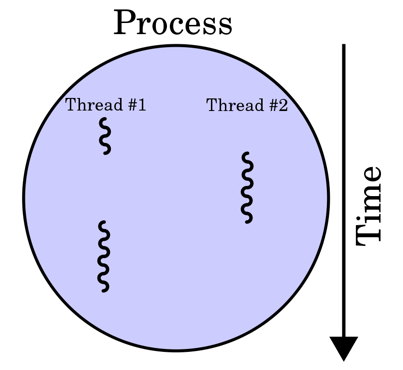
\includegraphics[width=0.4\linewidth]{images/midterm_2_solution_1.png}
            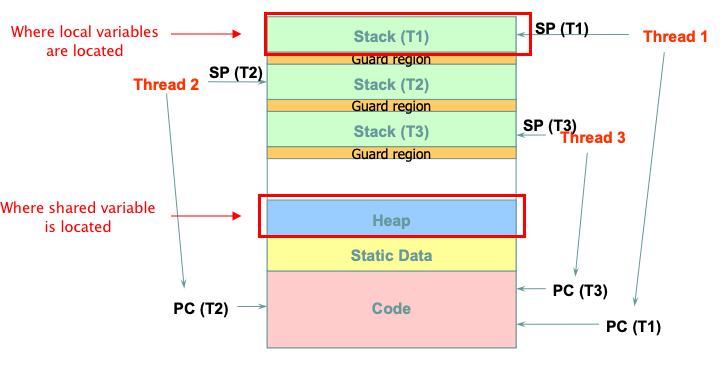
\includegraphics[width=\linewidth]{images/midterm_2_solution_2.png}
            \end{center}

            \item A thread is bound to a single process
            \item A process can have multiple threads
            \item Has two types
            \begin{itemize}
                \item \textbf{User-level Threads:}

                \begin{itemize}
                    \item Are implemented by users and kernel is not aware of the existence of these threads
                    \item Are represented by a program counter(PC), stack, registers and a small process control block
                    \item Are small and much faster than kernel level threads
                \end{itemize}
                \item \textbf{Kernel-level Threads:}

                \begin{itemize}
                    \item Are handled by the operating system directly
                    \item Thread management is done by the kernel
                    \item Are slower than user-level threads
                \end{itemize}
            \end{itemize}
        \end{itemize}

        \item \textbf{Process}

        \begin{itemize}
            \item Is a program in execution
            \item Is named by it's process ID or PID
            \item Can be described by the following states at any point in time

            \begin{itemize}
                \item Address Space
                \item CPU Registers
                \item Program Counter
                \item Stack Pointer
                \item I/O Information
            \end{itemize}

            (wait. this is PCB)

            \item Exists in one of many different \textbf{process states}, including

            \begin{enumerate}[1.]
                \item Running
                \item Ready to Run
                \item Blocked
            \end{enumerate}

            \bigskip

            \begin{itemize}
                \item Different events (Getting Scheduled, descheduled, or waiting for I/O)
                transitions one of these states to the other
            \end{itemize}

        \end{itemize}

        \item \textbf{Signals}

        \begin{itemize}
            \item Provides a way to communicate with the process
            \item Can cause job to stop, continue, or terminate
            \item Can be delivered to an application

            \begin{itemize}
                \item Stops the application from whatever its doing
                \item Runs Signal handler (some code in application to handle the signal)
                \item When finished, the process resumes previous behavior
            \end{itemize}
        \end{itemize}

        \item \textbf{Spinlock}
        \begin{itemize}
            \item Is the simplest lock to build
            \item Uses a lock variable

            \begin{itemize}
                \item 0 - (available/unlock/free)
                \item 1 - (acquired/locked/held)
            \end{itemize}

            \item Has two operations

            \begin{enumerate}[1.]
                \item \texttt{acquire()}

                \bigskip

                \begin{center}
                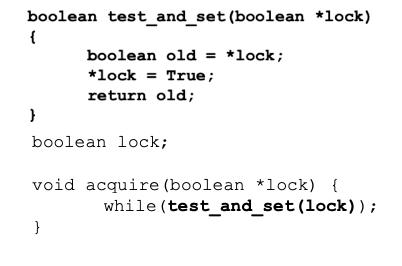
\includegraphics[width=0.7\linewidth]{images/midterm_2_solution_3.png}
                \end{center}

                \bigskip

                \item \texttt{release()}

                \bigskip

                \begin{center}
                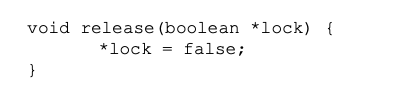
\includegraphics[width=0.7\linewidth]{images/midterm_2_solution_4.png}
                \end{center}

                \bigskip
            \end{enumerate}
            \item Allows a single thread to enter critical section at a time
            \item Spins using CPU cycles until the lock becomes available.
            \item May spin forever
        \end{itemize}

        \item \textbf{Scheduling policies}

        \begin{itemize}
            \item Are algorithms for allocating CPU resources to concurrent tasks
            deployed on (i.e., allocated to) a processor (i.e., computing resource)
            or a shared pool of processors $^{[5]}$
            \item Are sometimes called \textbf{Discipline}
            \item Covers the following algorithms in textbook

            \begin{itemize}
                \item \textbf{First In First Out}
                \item \textbf{Shortest Job First}
                \item \textbf{Shortest Time-to-completion First}
                \item \textbf{Round Robin}

                \begin{itemize}
                    \item Runs job for a \textbf{time slice} or \textbf{quantum}
                    \item Each job gets equal share of CPU time
                    \item Is clock-driven $^{[6]}$
                    \item Is starvation-free $^{[7]}$
                    \item \underline{Must} have the length of a time slice (\textbf{quantum}) as multiple of timer-interrupt period
                \end{itemize}

                \bigskip

                \begin{center}
                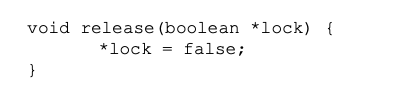
\includegraphics[width=0.7\linewidth]{images/midterm_2_solution_4.png}
                \end{center}
                \item \textbf{Multi-level Feedback Queue}
            \end{itemize}
        \end{itemize}

    \end{itemize}

    \bigskip

    \underline{\textbf{References}}

    \begin{enumerate}[1)]
        \item Coding Horror, Understanding User and Kernel Mode, \href{https://blog.codinghorror.com/understanding-user-and-kernel-mode/}{link}
        \item Kansas State University, Basics of How Operating Systems Work, \href{http://faculty.salina.k-state.edu/tim/ossg/Introduction/OSworking.html#:~:text=Interrupts%20are%20signals%20sent%20to,part%20of%20the%20operating%20system.&text=Hardware%20Interupts%20are%20generated%20by,some%20attention%20from%20the%20OS.}{link}
        \item Kansas State University, Glossary, \href{http://faculty.salina.k-state.edu/tim/ossg/glossary.html#term-context-switch}{link}
        \item Tutorials Point, User-level threads and Kernel-level threads, \href{https://www.tutorialspoint.com/user-level-threads-and-kernel-level-threads}{link}
        \item Science Direct, Scheduling Policy, \href{https://www.sciencedirect.com/topics/computer-science/scheduling-policy#:~:text=Scheduling%20policies%20are%20algorithms%20for,nature%20of%20applications%20%5B1%5D.}{link}
        \item Guru 99: What is CPU Scheduling?, \href{https://www.guru99.com/cpu-scheduling-algorithms.html#8}{link}
        \item Wikipedia: Round-robin Scheduling, \href{https://en.wikipedia.org/wiki/Round-robin_scheduling}{link}
    \end{enumerate}

    \item

    \begin{enumerate}[a)]
        \item
    \end{enumerate}

    \bigskip

    \underline{\textbf{Notes}}

    \begin{itemize}
        \item \textbf{System Call}

        \begin{itemize}
            \item Is the programmatic way in which a computer program requests a previleged service from the kernel of the operating system
            \item i.e. Reading from disk
            \item Steps

            \begin{enumerate}[1)]
                \item Setup \textbf{trap tables} on boot
                \item Execute system call
                \item Save \textit{Program Counter}, \textit{CPU registers}, \textit{kernal stack} (so process can resume after \textbf{return-from-trap}
                or \textbf{context switch})
                \item Switch from \textbf{user mode} to \textbf{kernel mode}
                \item Perform previleged operations
                \item Finish and execute \textbf{return-from-trap} instruction
                \item Return from \textbf{kernel mode} to \textbf{user mode} and resume user program
            \end{enumerate}
        \end{itemize}
    \end{itemize}
\end{enumerate}

\end{document}